\chapter{Исследовательская часть}

В данном разделе будут приведены примеры работы программа, а также проведен сравнительный анализ реализаций алгоритмов при различных ситуациях на основе полученных данных.

\section{Технические характеристики}

Технические характеристики устройства, на котором выполнялись замеры времени представлены далее:

\begin{itemize}
	\item операционная система Windows 11 Pro Версия 22H2 (22621.674) \cite{wind};
	\item память 16 ГБ;
	\item процессор 11th Gen Intel(R) Core(TM) i5-11400 2.59 ГГц \cite{proc}.
\end{itemize}

При тестировании компьютер был включен в сеть электропитания. Во время замеров процессорного времени устройство было нагружено только встроенными приложениями окружения, а также системой тестирования.

\section{Демонстрация работы программы}

На рисунке \ref{img:res} представлен результат работы программы. На экран выводятся результаты заемров времени для разных размеров матриц и разных видов алгоритмов матричного умножения в мс.
\newpage
%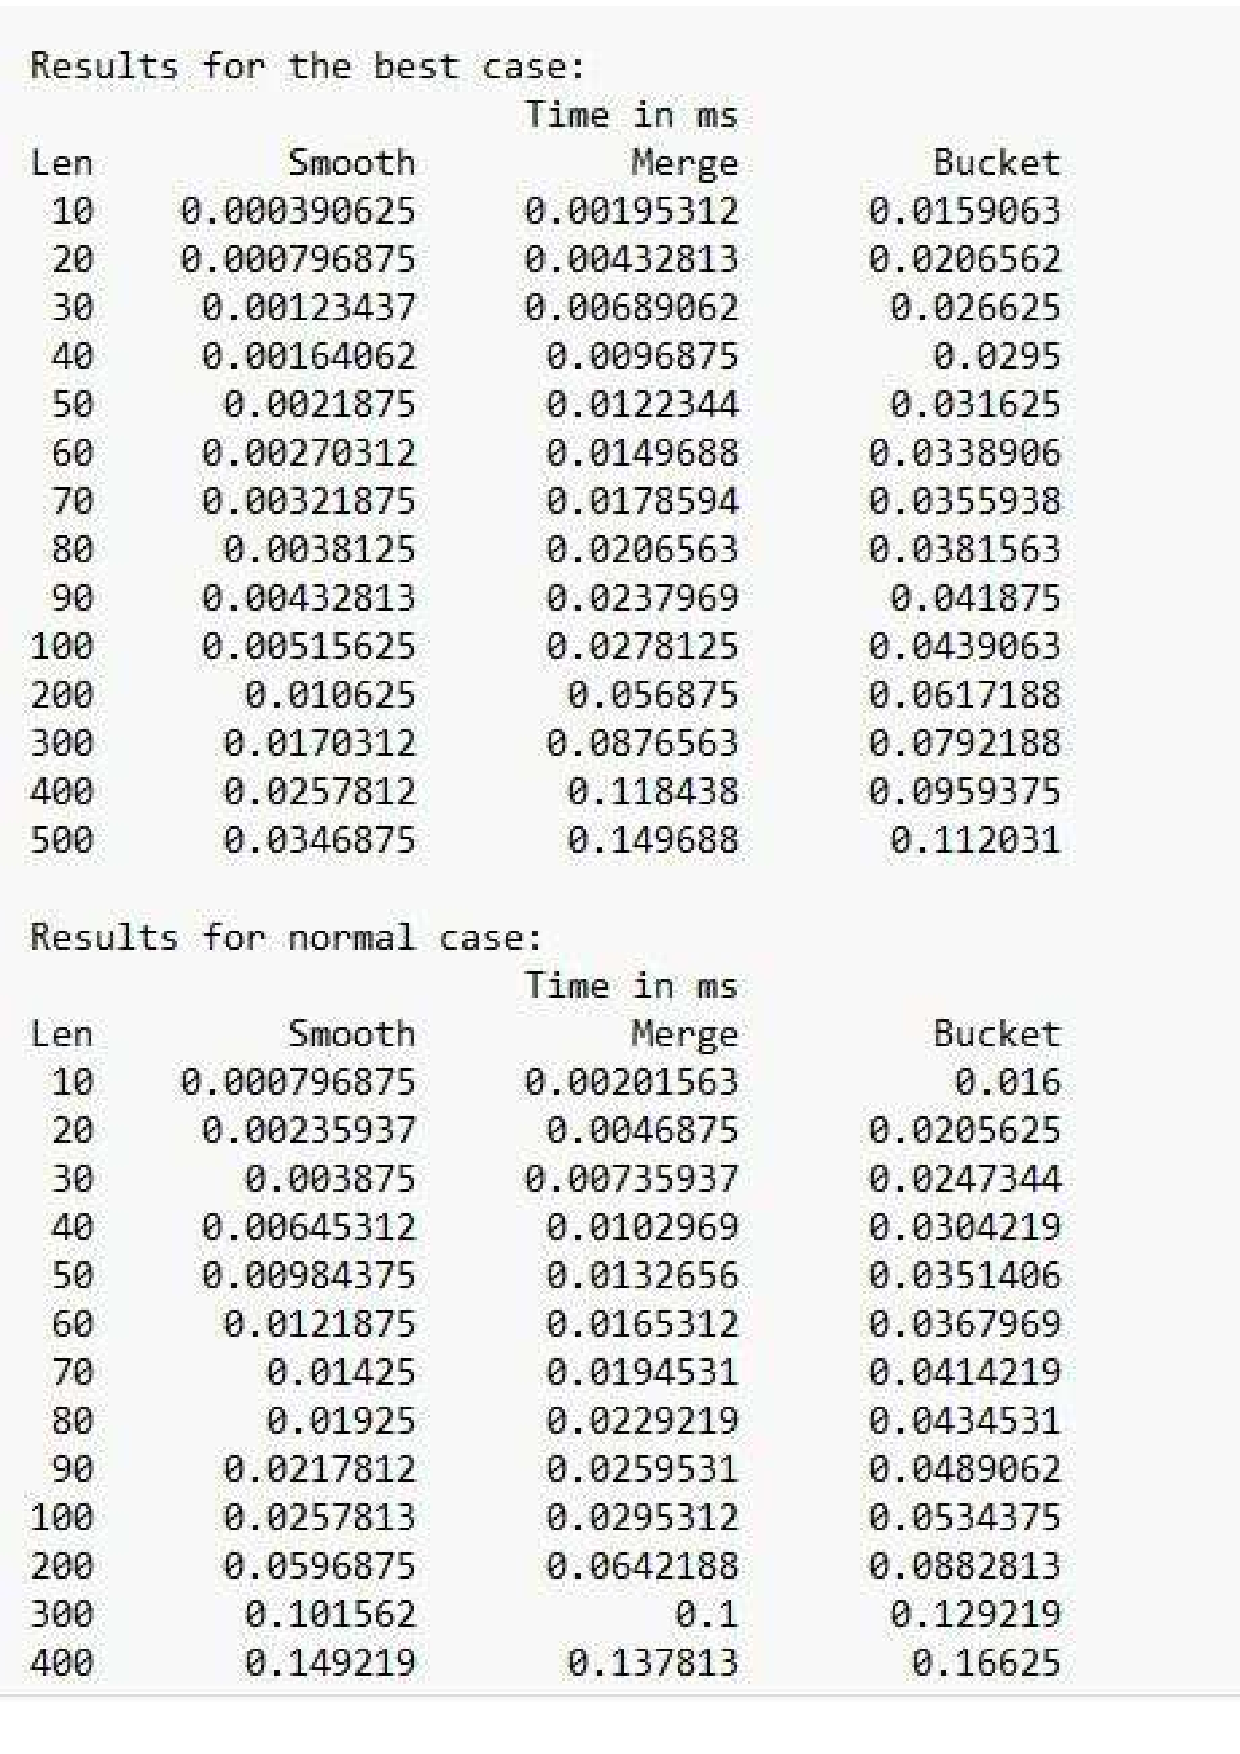
\includepdf[pages=-]{src/screen.pdf}
\begin{center}
	\centering{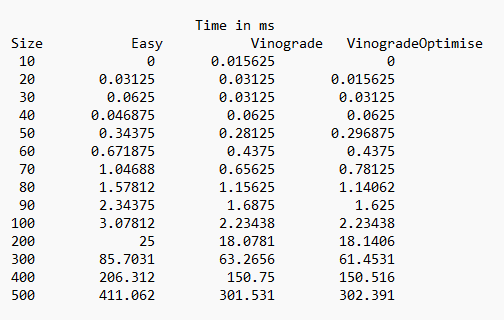
\includegraphics[trim=0 0 0cm 0cm bb=0 0 504 320]{src/screen}}
	\captionof{figure}{Пример работы программы}
	\label{img:res}
\end{center}

\section{Время выполнения реализаций алгоритмов}

Как было сказано выше, используется функция замера процессорного времени GetProcessTimes(...) из библиотеки Windows.h. Функция возвращает пользовательское процессорное временя типа float.

Использовать функцию приходится дважды, затем из конечного времени нужно вычесть начальное, чтобы получить результат.




\section*{Вывод}
\addcontentsline{toc}{section}{Вывод}


Теоретические результаты замеров и полученные практически результаты совпадают.